\chapter{\MakeUppercase{Инструменты для обнаружения взаимоблокировок}}

\section{Существующие решение}

Для обнаружения взаимоблокировок в программах, написанных на C и C++, на данный момент существуют данные решения:

\begin{itemize}  
\item Valgrind
\item Intel Parallel Studio
\item GDB с расширением для обнаружения взаимоблокировок
\item Google Thread Sanitizer
\end{itemize}

\subsection{Valgrind}

Valgrind \cite{ValgrindWiki} - инструмент для поиска ошибок при работе с п

\subsection{Intel Parallel Studio}

\subsection{GDB}

\subsection{Google Thread Sanitizer}

Google Thread Sanitizer - инструмент для нахождения ошибок в многопоточных приложения на C/C++ и Go. Позволяет находить гонки данных и детектировать возможные взаимные блокировки между потоками. К сожалению, GTSAN не может корректно обрабатывать все виды взаимных блокировок и имеет ошибки первого и второго рода.

\section{Алгоритм Google Thread Sanitizer}

Алгоритм Google Thread Sanitizer базируется на построение графа занятия ресурсов потоками.

\begin{figure}[htbp]
    \centering
    \begin{subfigure}[h]{0.4\textwidth}
        \centering
        \lstinputlisting[language=C]{inc/chapter-first/2m2t-dd.c}
    \end{subfigure}
    \hfill
    \begin{subfigure}[h]{0.4\textwidth}
        \centering
        \includegraphics[width=\textwidth]{inc/chapter-first/2m1t.eps}
    \end{subfigure}
    \caption{Фрагмент с взаимоблокировкой на двух потоках}
    \label{fig:2m2t-d}
\end{figure}

В процессе исполнения программы строится граф, вершинами которого являются мьютексы. В ходе исполнения потока строятся рёбра между последовательным захватом двух мьютексов. После построения графа производится поиск циклов, наличие которых говорит о deadlock. Однако алгоритм имеет ошибки первого и второго рода - ложное срабатывание и пропуск цели.

На Рис. \ref{fig:2m2t-d} происходит ошибка первого рода - ложное срабатывание. Поток, который первым захватит mu1, сможет без взаимной блокировки выполнить захват и освобождение остальных мьютексов, пока второй будет ожидать освобождения mu1. В цикле присуствует граф хотя взаимной блокировки не происходит.

\begin{figure}[htbp]
    \centering
    \begin{subfigure}[h]{0.4\textwidth}
        \centering
        \lstinputlisting[language=C]{inc/chapter-first/3m2t-du.c}
    \end{subfigure}
    \hfill
    \begin{subfigure}[h]{0.4\textwidth}
        \centering
        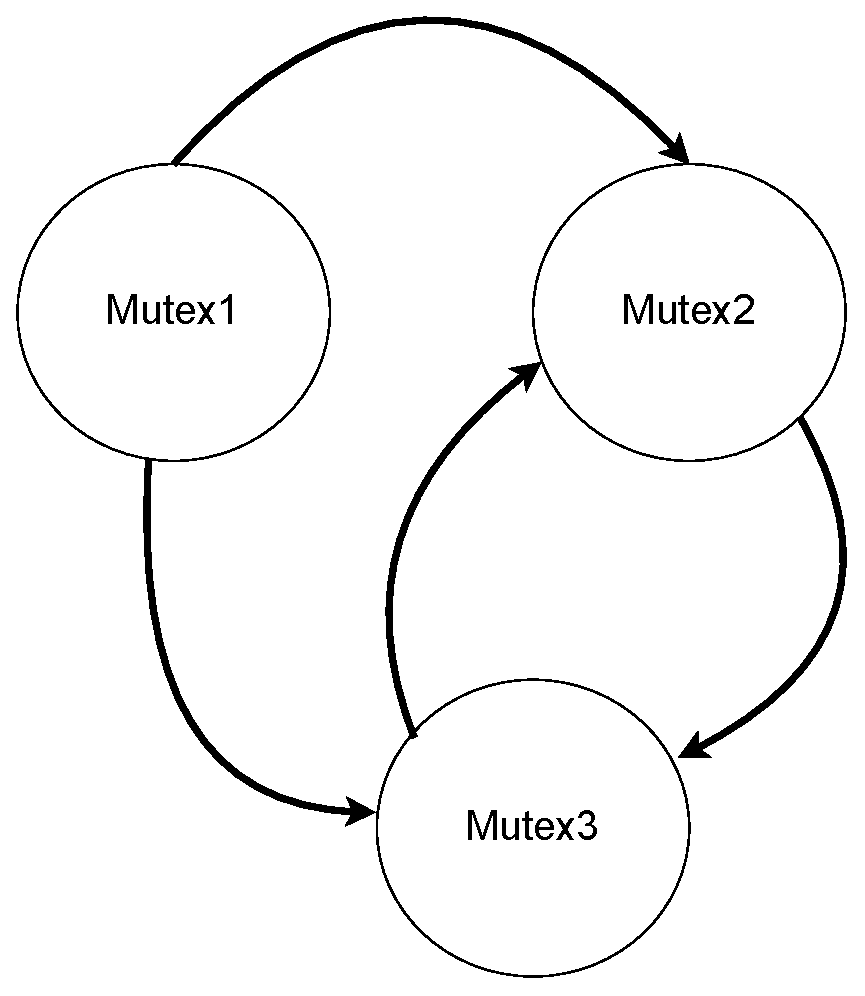
\includegraphics[width=\textwidth]{inc/chapter-first/3m2t-du.eps}
    \end{subfigure}
    \caption{Фрагмент программы с ложной взаимной блокировкой на трёх мьютексах}
    \label{fig:3m2t-du}
\end{figure}

Рассмотрим примеры с ошибкой второго рода - пропуск цели. На рис \ref{fig:2m2t-du} изображён один из возможных графов поиска взаимной блокировки. Код, который может вызвать взаимную блокировку, исполняется по случайному условию. В зависимости от значения функции rand() программа попадёт в ситуацию взаимной блокировки. Данный алгоритм не может обнаружить случаи, которые происходят в возможных ветвлениях программы.


\begin{figure}[htbp]
    \centering
    \begin{subfigure}[h]{0.4\textwidth}
        \centering
        \lstinputlisting[language=C]{inc/chapter-first/2m2t-du.c}
    \end{subfigure}
    \hfill
    \begin{subfigure}[h]{0.4\textwidth}
        \centering
        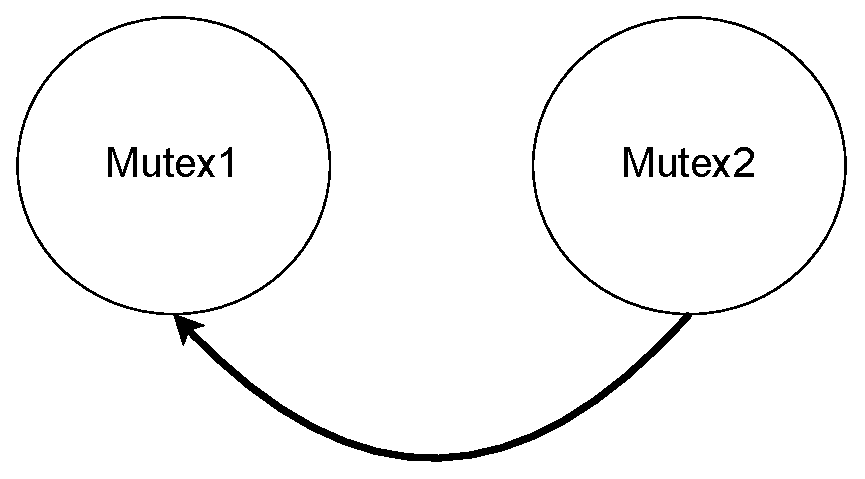
\includegraphics[width=\textwidth]{inc/chapter-first/2m2t-du.eps}
    \end{subfigure}
    \caption{Фрагмент программы с возможным пропуском возможной взаимной блокировки}
    \label{fig:2m2t-du}
\end{figure}

На Рис. \ref{fig:1m1t-d} происходит блокировка на одном потоке, что не обнаруживает Google thread sanitizer.

\begin{figure}[htbp]
\lstinputlisting[language=C]{inc/chapter-first/1m1t.c}
 \caption{Фрагмент программы с взаимоблокировкой на одном потоке}
 \label{fig:1m1t-d}
\end{figure}

При этом Google TSAN и Valgrind не способны обнаружить Deadlock, который произошел уже во время исполнения программы, поэтому в случае возникновения блокировки может быть неясно - это программа долго выполняется или произошёл Deadlock.

\subsection{PostgreSQL}

В PostgreSQL реализован алгоритм автоматического обнаружения Deadlock\cite{ref_postgre_deadlock}. Рассмотрим пример выполнения двух процессов, приведенный на Рис.~\ref{fig:postgre-flow}.

\begin{figure}[h]
\begin{lstlisting}[language=SQL]
process A: BEGIN;

process B: BEGIN;

process A: UPDATE users SET name = "Peter" WHERE id = 1;

process B: UPDATE users SET name = "Marko" WHERE id = 2;

process A: UPDATE users SET name = "John" WHERE id = 2;

process B: UPDATE users SET name = "John" WHERE id = 1;
\end{lstlisting}
\caption{PostgreSQL flow} 
\label{fig:postgre-flow}
\end{figure}

В данном случае процесс A блокирует запись с идентификатором id = 1, а процесс B блокирует запись с идентификатором id = 2. После чего процесс B пытается изменить запись, которую заблокировал процесс A c id = 1, и ждёт пока процесс A завершиться. Аналогичная ситуация происходит и с процессом A, после чего процессы находятся во взаимной блокировке.

PostgreSQL распознает ситуацию, когда два процесса блокируют другу друга, ожидает в течении некоторого интервала времени, после чего выводит ошибку.

\clearpage